% Preamble
\documentclass[12pt, aspectration=169]{beamer}
\usetheme{Copenhagen}
\usecolortheme{beaver}

\setbeamertemplate{navigation symbols}{}

% Packages
\usepackage{amsmath}
\usepackage{listings}
\usepackage{xcolor}
\usepackage{blkarray}
\usepackage{graphicx}
\usepackage{hyperref}

\definecolor{codegreen}{rgb}{0,0.6,0}
\definecolor{codegray}{rgb}{0.5,0.5,0.5}
\definecolor{codepurple}{rgb}{0.58,0,0.82}
\definecolor{backcolour}{rgb}{0.95,0.95,0.92}

\lstdefinestyle{mystyle}{
    backgroundcolor=\color{backcolour},
    commentstyle=\color{codegreen},
    keywordstyle=\color{magenta},
    numberstyle=\tiny\color{codegray},
    stringstyle=\color{codepurple},
    basicstyle=\ttfamily\footnotesize,
    breakatwhitespace=false,
    breaklines=true,
    captionpos=b,
    keepspaces=true,
    numbers=left,
    numbersep=5pt,
    showspaces=false,
    showstringspaces=false,
    showtabs=false,
    tabsize=4
}

\lstset{style=mystyle}

\title{Introduction to Advanced Python:\\Why is Python slow?}
\author{Kai Striega}
\date{\today}

% Document
\begin{document}

    \maketitle

    \begin{frame}{Before I start}
        \begin{block}{Here be dragons}<2->
            This talk introduces advanced topics, quickly.
            The content is designed to stretch your understanding and to challenge you.
        \end{block}
        \begin{block}{Questions}<3->
            I am happy to take questions during the talk, feel free to ask if something doesn't make sense.
        \end{block}
    \end{frame}

    \begin{frame}{What we're going to do today}
        \begin{itemize}
            \item<2-> Answer the question: Why is Python slow?
            \item<3-> Compare Python to C and assembly
            \item<4-> Introduce some of the key ideas in performance analysis
            \item<5-> Discuss when execution time matters\ldots and when it doesn't
        \end{itemize}
    \end{frame}

    \begin{frame}{Why C?}
        \begin{columns}
            \column{0.55\textwidth}
            \begin{itemize}
                \item C is \textit{very} fast
                \item CPython is written in C
                \item Many Python extensions are written in C
            \end{itemize}
            \column{0.45\textwidth}
            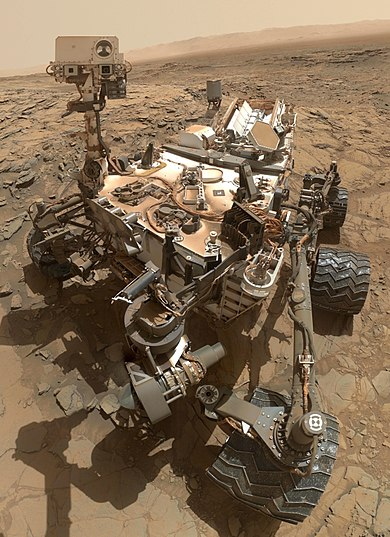
\includegraphics[scale=0.35]{static/images/390px-Curiosity_Self-Portrait_at_'Big_Sky'_Drilling_Site}
        \end{columns}
    \end{frame}
    \begin{frame}{Today's Example}
        \lstinputlisting[language=Python,label={lst:python}]{code/sum_of_first_n_numbers.py}
    \end{frame}

    \begin{frame}{Is Python slow?}
        \begin{itemize}
            \item[]<2-> \texttt{time python sum\_of\_first\_n\_numbers.py\newline}
            \item[]<3-> \texttt{total=18446744064889498501\newline
            real 5m56.581s\newline
            user 5m56.518s\newline
            sys 0m0.004s\newline}
        \end{itemize}
    \end{frame}

    \begin{frame}{Today's Example, but in C}
        \lstinputlisting[language=C,label={lst:C}]{code/sum_of_first_n_numbers.c}
    \end{frame}

    \begin{frame}{What about C?}
        \begin{itemize}
            \item[]<2-> \texttt{time bin/sum\_of\_first\_n\_numbers\_O3\newline}
            \item[]<3-> \texttt{total=18446744064889498501\newline
            real 0m0.000s\newline
            user 0m0.000s\newline
            sys 0m0.000s\newline}
        \end{itemize}
    \end{frame}

    \begin{frame}{Why?}
        \begin{itemize}
            \item \textit{0m0.000s} seems like a bug\ldots but it's not!
            \item C is a \textbf{compiled} langauge
            \item That means the compiler can perform optimizations before the code is run
        \end{itemize}
    \end{frame}

    \begin{frame}{Assembly}
        \begin{itemize}
            \item I'm about to show you a language called \textit{Assembly}
            \item Assembly corresponds to the CPU's machine instructions
            \item a.k.a.\ the instructions the CPU is executing
            \item Assembly is specific to your CPU architecture
        \end{itemize}

        \begin{alertblock}{Assembly}<2->
            Assembly is a new topic that you (probably) won't have to know in depth.
            It is included here to analyse the code being run by C, but you won't have to remember the in and outs of
            assembly.
        \end{alertblock}
    \end{frame}

    \begin{frame}{What C does}
        \lstinputlisting[label={lst:asm-O3-no-arg}]{static/code/sum_clang_17_O3.asm}
    \end{frame}

    \begin{frame}{Today's Example, in C, with arguments}
        \lstinputlisting[language=C,label={lst:C-args}]{code/sum_of_first_n_numbers_arg.c}
    \end{frame}

    \begin{frame}{What about with an argument?}
        \begin{itemize}
            \item[]<2-> \texttt{time bin/sum\_of\_first\_n\_numbers\_arg\_O3\newline}
            \item[]<3-> \texttt{total=18446744064889498501\newline
            real 0m0.000s\newline
            user 0m0.000s\newline
            sys 0m0.000s\newline}
        \end{itemize}
    \end{frame}

    \begin{frame}{What C does (with an argument)}
        \lstinputlisting[label={lst:asm-O3-arg}]{static/code/sum_arg_clang_17_O3.asm}
    \end{frame}

    \begin{frame}{What has the compiler done for me lately?}
        \begin{itemize}
            \item There's an alternate way to calculate the sum of the first $n$ numbers
            \item $\frac{n(n + 1)}{2}$
            \item The compiler transformed the algorithm from one with linear runtime to constant runtime
        \end{itemize}
    \end{frame}

    \begin{frame}{What C does (without optimizations)}
        \lstinputlisting[label={lst:asm-O3-arg-O0}]{static/code/sum_arg_clang_17_O0.asm}
    \end{frame}

    \begin{frame}{What if we don't use optimizations?}
        \begin{itemize}
            \item[]<2-> \texttt{time bin/sum\_of\_first\_n\_numbers\_arg\_O0\newline}
            \item[]<3-> \texttt{total=18446744064889498501\newline
            real 0m2.020s\newline
            user 0m2.010s\newline
            sys 0m0.010s\newline}
        \end{itemize}
    \end{frame}

    \begin{frame}{What we've done so far}
        \begin{itemize}
            \item We've turned a 6-minute problem into a 2-second problem
            \item By changing the language
            \item This speedup exists even without optimizations
        \end{itemize}
    \end{frame}

    \begin{frame}{What makes C so much faster than Python?}
        \begin{description}
            \item[Interpreted vs Compiled] Python is \textit{interpreted} $\implies$ CPU has to do extra work to translate the code at runtime
            \item[Memroy Access Patterns] Python stores everything in a \textit{PyObject} this means the CPU can't access data as efficiently
        \end{description}
    \end{frame}

    \begin{frame}{What does it take to run Python?}
        \begin{description}
            \item[Source Code] You start with a Python source code file (typically ending in .py) that contains the instructions you want the computer to execute.
            \item[Tokenizer] The source code is read by the Python interpreter, which breaks it down into a series of tokens.
            \item[Parser] This is where the interpreter checks if the arrangement of tokens conforms to the rules of the Python language.
        \end{description}
    \end{frame}

    \begin{frame}{What does it take to interpet Python?}
        \begin{description}
            \item[AST] An AST is a hierarchical representation of the program's structure.
            The nodes of the tree represent operations, while the edges represent control flow.
            \item[Semantic Analysis] The interpreter now checks the AST for semantic correctness.
            \item[Execution] The Python interpreter executes the code by walking through the AST and performing the operations specified by the source code.
        \end{description}
    \end{frame}

    \begin{frame}{What limits the performance of a CPU?}
        \begin{description}
            \item[Memory Bound] How quickly we can get data to the CPU
            \item[CPU Bound] How quickly the CPU can execute instructions
        \end{description}
    \end{frame}

    \begin{frame}{Memory Latencies}
        \begin{center}
            \begin{tabular}{|c c|}
             \hline
              & Latency \\ [0.5ex]
             \hline\hline
             L1 Cache & $<$1ns \\
             \hline
             L2 Cache & 4ns \\
             \hline
             Main Memory & 100ns \\
             \hline
             SSD & 16 $\mu$s \\ [1ex]
             \hline
             Round Trip (Datacenter)   & 0.5ms     \\
             \hline
             Round Trip (US to Europe) & 150 ms \\ [1ex]
             \hline
            \end{tabular}
        \end{center}
    \end{frame}

    \begin{frame}{Memory Latencies}
        \begin{center}
            \begin{tabular}{|c c|}
             \hline
              & Latency \\ [0.5ex]
             \hline\hline
             L1 Cache & $<$1 second \\
             \hline
             L2 Cache & 4 seconds \\
             \hline
             Main Memory & 100 seconds \\
             \hline
             SSD & 4.5 hours \\ [1ex]
             \hline
             Round Trip (Datacenter)   & 5.8 days     \\
             \hline
             Round Trip (US to Europe) & 5 years \\ [1ex]
             \hline
            \end{tabular}
        \end{center}
    \end{frame}

    \begin{frame}{Further Reading}
        \begin{itemize}
            \item \url{https://computers-are-fast.github.io/}
            \item \url{https://colin-scott.github.io/personal_website/research/interactive_latency.html}
        \end{itemize}
    \end{frame}

\end{document}